\documentclass[output=paper]{LSP/langsci}
\ChapterDOI{10.5281/zenodo.1407025}
\author{Jana Strnadová\affiliation{Google, inc.}}
\title{Lexeme equivalence or rivalry of lexemes?}
\subtitle{On the purported interchangeability between French nouns and denominal adjectives}
\abstract{This paper deals with the purported interchangeability between nouns and adjectives derived from nouns in French. The question of equivalence or rivalry between a morphologically complex adjective and a syntactic construction containing a morphologically-related noun links a field of studies on rivalry between inflected word forms, derivational suffixes or different syntactic constructions to express the same meaning. This paper then presents a corpus-based study of the relative distribution of nominal or adjectival realizations of a modifier of the same head noun and discusses some motivations that play a role in the choice of one or the other strategy.}


\maketitle


\begin{document}
\selectlanguage{english}


\section{Introduction}

Both in syntax and in morphology, the same  content can be expressed by different structural means.

In syntax, this may take the form of valency alternations such as the English dative alternation (e.g. \emph{Mary gave a watch to me} vs. \emph{Mary gave me a watch}) or of word order alternations such as exemplified by the position of French attributive adjectives with respect to their governing noun. Such alternations have been the focus of much attention in the recent literature which focuses on establishing the interplay of various non-categorical factors (see e.g. \citealt{bresnan2007}  on the dative alternations, \citealt{thuilier2012}  on French adjectives).

In morphology, the consensus has long been that such alternations are inexistent or unexpected: in inflection, a unique form was assumed to fill each cell of a lexeme's paradigm \citep{Anderson92, Stump01}, in word formation, rivalry between affixes was taken to be resolved by blocking \citep{Aronoff1976}. This consensus has progressively collapsed in the last two decades. Under the impulsion of \citet{Thornton12}, the phenomenon of overabundace, where multiple forms fill a paradigm cell, has become a central issue in inflectional morphology (see e.g. \citealt{bermel} for Czech noun declension, \citealt{Stump16}, Bonami \& Crysmann this volume, Thornton this volume). Likewise, situations of non-categorical competition between derivational processes have moved from the fringes \citep{rainer1988, Plag1999} to the center of  attention for derivational morphologists \citep{Lindsay2013, villoing2009vn,Tribout2010a, fradin2012moyen, koehl2012, namer2013, strnadova2014}.

In this paper, I focus on situations of alternation between the morphological or syntactic expression of some content. This is familiar in the context of inflection where overabundance between synthetic and periphrastic expression of paradigm cells is well-documented \citep{aronofflindsay2014, bonami2015}. For example, \emph{friendlier} and \emph{more friendly} are both realizations of the comparative degree of the lexeme \lxm{friendly}. Situations in which a syntactic construction and a derivational process led to the expression of the same content have been comparatively less studied.\footnote{In French, for example, the topic of possible competition between morphologically complex words and syntactic phrases has been studied for causative verbs \citep{dalnamer2003cause}.} Here I will specifically examine the expression of  nominal modification by a prepositional phrase containing some noun N or a denominal adjective derived from that same noun. This is illustrated in (\ref{ex:Strnadova:faute grammaticale}): the adjective \emph{grammaticale} in (\ref{ex:Strnadova:grammaticale}) and the noun \emph{grammaire} introduced by the preposition \emph{de} in (\ref{ex:Strnadova:grammaire}) roughly make  the same contribution.

\begin{exe}
\ex \label{ex:Strnadova:faute grammaticale} \begin{xlist}
	\ex \label{ex:Strnadova:grammaticale} {faute grammaticale}\\ `grammatical mistake'
	\ex \label{ex:Strnadova:grammaire} {faute de grammaire}\\ `grammar mistake'
	\end{xlist}
\end{exe}

The central questions that arise in view of such examples are 1) to what extent can the adjective and the prepositional phrase be taken to be semantically equivalent and 2) whether the two constructions should be taken to be paradigmatic alternatives in the same way as \emph{friendlier} and \emph{more friendly} are.


\section{Background and methodology}

The proximity between a denominal adjective and a prepositional phrase containing a morphologically related noun was observed as early as \citet[413]{dumarsais}: ``When there is a simple preposition \emph{de}, without an article, the preposition and its complement are considered adjectively. \emph{Un palais de roi}, is equivalent to \emph{palais royal} `royal palace'; \emph{une valeur de héros} equals to \emph{une valeur héroïque} `heroic value'."\footnote{Orig. ``Lorsqu'il n'y a qu'une simple préposition \emph{de}, sans l'article, la préposition et son complément sont pris adjectivement. \emph{Un palais de roi}, est équivalent à un \emph{palais  royal}; \emph{une valeur de héros} équivaut à \emph{une valeur héroïque}."} \citet{bally} used the term \emph{transpositions} and \citet{tesniere} called this kind of adjectivisation \emph{translations}.

The idea of equivalence between the two constructions was discussed later for example by \citet{bosredon1988} or  \citet{bartnoailly1993},  or in a more semantic approach, by \citet{nowakowska2004} and \citet[380]{roche2006adj}, who insists on the equivalence by describing ``the adjectivized noun lexically as it can be syntactically with the preposition de".\footnote{Orig. ``le nom adjectivé lexicalement comme il peut l'être syntaxiquement par la préposition de".}

Functional and semantic equivalence between a denominal adjective and its base noun used in a prepositional phrase is thus considered as one of the characteristics of denominal adjectives. The examples (\ref{ex:Strnadova:faute grammaticale})-(\ref{ex:Strnadova:famille-équivalence}) show the possibility to substitute a derived adjective with a prepositional phrase.

\begin{exe}
\ex \begin{xlist} \label{ex:Strnadova:de-équivalence}
\ex {le climat social}\\ `social climate'
\ex {le climat de la société}\\ `climate of the society'
\end{xlist}
\end{exe}
\begin{exe}
\ex \label{ex:Strnadova:famille-équivalence} \begin{xlist}
\ex {secret de famille}\\ `family secret'
\ex {secret familial}\\ `family secret'
\end{xlist}
\end{exe}

The question is then to what extent are prepositional phrases functionally and semantically equivalent to denominal adjectives in French? This question was of central importance in the 1980s and 1990s. At that time, the interest focused on the argument realization of the head noun with the goal of defining the syntactic and semantic relations within a noun phrase (\citealt{bartning1980, pinchon1980, monceaux1993}, etc.). These works showed that adjectives and prepositional phrases are not equivalent and are not interchangeable without any restriction.

More recently, \citet{cartonideleger2010} studied the use of an adjective or of its corresponding prepositional phrase in specialized or general medical corpora and showed that there is a preference for the use of adjectives in specialized texts, while corresponding prepositional phrases are more frequent in non-specialized texts (\ref{ex:Strnadova:rythme-cardiaque}).


\begin{exe}
\ex \begin{xlist}\label{ex:Strnadova:rythme-cardiaque}
\ex {rythme cardiaque}\\ `cardiac rhythm'
\ex {rythme du c{\oe}ur}\\  `heart rhythm'
\end{xlist}
\end{exe}

Finally, \citet{boledaevert2012} provided some statistical evidence supporting the claim that an ethnic adjective, which is in a certain way a denominal adjective, cannot be interpreted as the argument of the noun as in (\ref{ex:Strnadova:accord français}). The adjective acts as a simple modifier. In their study, the modified noun is a predicative noun.

\begin{exe}
\ex \begin{xlist}  \label{ex:Strnadova:accord français}
\ex {French agreement}
\ex {agreement by France}
\end{xlist}
\end{exe}


All these studies have one thing in common: they do not differentiate between cases where the prepositional phrase contains a fully determined NP and those where it contains just a bare noun. In (\ref{ex:Strnadova:décision-gouvernement}), the adjective \emph{gouvernementale}  is in competition with the prepositional phrase containing a definite noun phrase (\emph{le gouvernement}\footnote{The definite article \emph{le} is merged with the preposition \emph{de} which results in \emph{du gouvernement}.}), while in (\ref{ex:Strnadova:campagne-publicitaire}), the preposition governs a bare noun (\emph{publicité}). Semantically, in (\ref{ex:Strnadova:décision-gouvernement}), the noun phrase within the PP refers to the cabinet, while the noun phrase in (\ref{ex:Strnadova:campagne-publicitaire}) doesn't refer to an advertisement.

 
\begin{exe}
\ex \begin{xlist} \label{ex:Strnadova:décision-gouvernement}
	\ex {décision gouvernementale}\\  `governmental decision'
	\ex {décision du gouvernement}\\ `the government's decision'
	\end{xlist}
\ex  \begin{xlist} \label{ex:Strnadova:campagne-publicitaire}
	\ex {campagne publicitaire}\\ `advertising campaign'
	\ex {campagne de publicité}\\ `advertising campaign'
	\end{xlist}
\end{exe}

Contrary to these previous studies, I examine denominal adjectives and their syntactic equivalents with the restriction on prepositional phrases containing a bare noun introduced by the preposition \emph{de}. In such cases, the noun does not head a referential expression. Note that this restriction entails that the investigation be limited to cases where the adjective is derived from a common noun, as exemplified in (\ref{ex:Strnadova:paire-publicité}). Adjectives derived from proper names are excluded   since the proper names being definite noun phrases are referential expressions.

\begin{exe}
\ex  \label{ex:Strnadova:paire-publicité} {campagne de publicité / publicitaire}
\end{exe}

Three situations must be distinguished concerning the availability of a denominal adjective corresponding to a French noun: (i) there is an adjective regularly derived from a noun (\ref{ex:Strnadova:regul}); (ii) there is an adjective with a formal mismatch in comparison with the noun (\ref{ex:Strnadova:mismatch}); (iii) there is no adjective (\ref{ex:Strnadova:no-a-N2}) and hence a prepositional phrase is the only possible realization of the modifier (\ref{ex:Strnadova:ex-no-a-PP}).

\begin{exe}
\ex \label{ex:Strnadova:regul} \lxm{publicité} `advertisement' $\rightarrow$ \lxm{publicit-aire} `advertising'
\end{exe}

\begin{exe}
\ex  \label{ex:Strnadova:mismatch} \lxm{langue} `language' \rel  \lxm{linguistique} / $\ast$\lxm{languique}
\end{exe}

\begin{exe}
\ex \label{ex:Strnadova:no-a-N2} \begin{xlist}
\ex \lxm{décollage} `take-off' $\rightarrow$ ?
\ex \lxm{arrivée} `arrival' $\rightarrow$ ?
\ex \lxm{secours} `emergency' $\rightarrow$ ?
\end{xlist}
\end{exe}

\begin{exe}
\ex  \label{ex:Strnadova:ex-no-a-PP} \begin{xlist}
\ex {piste de décollage}\\ `runway'
\ex {hall d'arrivée}\\ `arrival hall'
\ex {issue de secours}\\ `emergency exit'
\end{xlist}
\end{exe}

It is notable that languages differ in this respect. As Table \ref{tab:Strnadova:compar-langues} shows, Czech tends to have available denominal adjectives where French does not. English has the same gap as French but uses compounding rather than PP modifications as an alternative strategy.

\begin{table}

\begin{tabularx}{.8\textwidth}{lX@{\qquad}ll@{\qquad}c }
\lsptoprule
\multicolumn{2}{l}{\hspace*{5mm}French}& \multicolumn{2}{l}{\hspace*{5mm}Czech} &English\\
{$N_1$}& ~~{$deN_2$}&~~{$A_d$}& ~~{$N_1$}& $N_2N_1$\\
\midrule
\emph{hall} &\emph{d'arrivée}& \emph{p\v{r}\'{i}jezdov\'{a}}& \emph{hala} & \emph{arrival hall}  \\
\emph{issue} &\emph{de secours}&\emph{nouzov\'{y}}&\emph{v\'{y}chod}& \emph{emergency exit}\\
\emph{carte}& \emph{de crédit}&\emph{kreditn\'{i}}& \emph{karta}& \emph{credit card}\\
\emph{piste} &\emph{de décollage}& \emph{vzletov\'{a}}& \emph{dr\'{a}ha}& \emph{runway} \\
\lspbottomrule
\end{tabularx}
\caption{Comparison between French, Czech and English noun phrases}
\label{tab:Strnadova:compar-langues}
\end{table}

To study the rivalry between  denominal adjectives and prepositional phrases, the following resources were used:
\begin{enumerate}
\item A lexicon of noun-adjective pairs  from \emph{DenALex} \citep{strnad2011} and \emph{Lexique3} \citep{new2006lexique}. 5,888 noun-adjective pairs with regularly derived adjectives
and 234 noun-adjective pairs with a formal mismatch were obtained in this way.
\item The corpus \emph{Est républicain} which covers three years of a local newspaper (1999, 2002, 2003) and contains 119.5 million word tokens with morphosyntactic annotation \citep{seddah2012}.
\end{enumerate}
Table \ref{tab:Strnadova:33} illustrates the diversity of denominal adjectives contained in the lexicon.

\begin{table}
\begin{tabularx}{.8\textwidth}{Xll}
\lsptoprule
Suffix &Noun &Adjective\\
\midrule
\emph{-aire}&\lxm{cellule} `cell'&\lxm{cellulaire} `cellular'\\
\emph{-al}&\lxm{parent} `parent' &\lxm{parental} `parental'\\
\emph{-el}&\lxm{culture} `culture' &\lxm{culturel} `cultural'\\
\emph{-esque}&\lxm{carnaval} `carnival' &\lxm{carnavalesque} `of carnival'\\
\emph{-eux}&\lxm{angine} `angina'&\lxm{angineux} `anginal'\\
\emph{-ien}&\lxm{microbe} `microb'&\lxm{microbien} `microbial'\\
\emph{-ier}&\lxm{côte} `coast' &\lxm{côtier} `coastal'\\
\emph{-ique}&\lxm{méthode} `method'&\lxm{méthodique} `methodical'\\
\emph{-u}&\lxm{feuille} `leaf' &\lxm{feuillu} `leafy'\\
\lspbottomrule
\end{tabularx}
\caption{Sample of French Denominal Adjectives}
\label{tab:Strnadova:33}
\end{table}

The following methodology was applied: search in the corpus for all combinations where a noun is followed by an adjective from the lexicon or by a prepositional phrase with \emph{de} containing a noun from the lexicon (\ref{ex:Strnadova:pair-public}).

\begin{exe}
\ex \label{ex:Strnadova:pair-public} \begin{xlist}
\ex lexicon entry: \lxm{publicité - publicitaire}  `advertisment - advertising'
\ex corpus search$_1$: X$_N$ {publicitaire}
\ex corpus search$_2$: X$_N$ {de publicité}
\ex search result: {campagne de publicité, campagne publicitaire, etc.}
\end{xlist}
\end{exe}

The vocabulary used throughout this article can be defined as follows: $N_1$  is the modified noun or the head noun. $A_d$ is the modifying denominal adjective. $N_2$ is the noun morphologically related to the adjective $A_d$. The term \emph{combination} stands for the search results $N_1 A_d$ and $N_1deN_2$. In each combination,  $deN$ stands for the nominal realization and $A_d$ for the adjectival realization of the modifying concept $N$.

For each triple $\langle N_1,A_d,N_2\rangle$, I computed the frequency $F_1$ of the $N_1A_d$ of the noun-adjective sequence, the frequency  $F_2$ of the $N_1deN_2$ sequence, their sum frequency $\emph{SumFreq}=F_1+F_2$ and the relative frequency of the $N_1A_d$ sequence, $\emph{Rfreq}=\frac{F_1}{\emph{SumFreq}}$. For instance,  for the triple $\langle\textrm{campagne, publicitaire, publicité}\rangle$, the corpus contains 40 occurrences of \emph{campagne publicitaire} and 27 occurrences of \emph{campagne de publicité}; hence $\emph{SumFreq}=67$ and $\emph{Rfreq}=\frac{40}{40+27}\approx 0.6$.

\section{Corpus-based results}

A first study focused on the pairs containing a regular denominal adjective, i.e. there is no formal mismatch between the noun and the adjective except for the suffix. 139,838 types of combinations (out of 1,137,137 occurrences) were collected. 45\% of nouns (2,686 lexemes) from the lexicon were attested in the corpus. Likewise, 30\% of adjectives (1,708 lexemes) were attested. Incomplete attestation was to be expected, since the lexicon contains many scientific terms which are not found in a journalistic corpus and many types have a very low frequency anyway.

The data distribution is presented in Table \ref{tab:Strnadova:nb}.

\begin{table}
\begin{center}
\begin{tabular}{lrrrrl}
\lsptoprule
\emph{SumFreq}&\multicolumn{1}{c}{All}&\multicolumn{1}{c}{Only $N_1A_d$}& \multicolumn{1}{c}{Only $N_1deN_2$}&\multicolumn{1}{c}{Both}&\%\\
\midrule
$\geq$0&139,838&70,876&63,145&\lgc{5,817}&=\lgc{4\%}\\
$\geq$10&13,422&6,175&4,986&\lgc{2,261}&=\lgc{17\%}\\
$\geq$100&1,586&687&535&\lgc{364}&=\lgc{23\%}\\
$\geq$1000&100&45&29&\lgc{26}&=\lgc{26\%}\\
\lspbottomrule
\end{tabular}
\end{center}
\caption{ Type counts of $N_1A_d$ and $N_1deN_2$ combinations by sum token frequency of the triple}
\label{tab:Strnadova:nb}
\end{table}

There is an inverse correlation between the token frequency of the triple (\emph{SumFreq}) and the proportion of cases where both strategies are attested. In particular, whereas only 4\% of triples are attested in both strategies overall, this proportion rises to 26\% for triples with a \emph{SumFreq} above 1,000.

For the rest of the study, only the types with a sum frequency above 10 were taken into account. At this threshold, there are 17\% of cases which can be realized either as an adjective or as a prepositional modifier and which are then possible rivals. This corresponds to 937 different nouns covering 16\% of the lexicon and  659 adjectives corresponding to 11\% of the lexicon.

\newpage 
46\% of cases only have an adjectival realization for the same head noun and 37\% of combinations only have the nominal realization. This leads to a U-shaped distribution with many cases at the edges and few cases in the middle of the distribution, what \citet{zuraw} calls a ``polarized distribution". If denominal adjectives and prepositional phrases were in free variation, then many more cases would be expected in the middle of the distribution.

Table \ref{tab:Strnadova:distr-rel-freq} shows the number of types in each interval of the distribution. As can be seen, many cases have a strong preference for one or the other realization. There are only 154 types with a relative frequency between 0.4 and 0.6, which could be described as real cases of free variation. I will call pairs having such a distribution \emph{strong rivals}.

\begin{table}

\begin{tabular}{cccc}
\lsptoprule
\emph{Rfreq} interval &\% of data&\# of types&\\
\midrule
0 < Rfreq < 1 & 17\%&2,261 types&\\
0.2 < Rfreq < 0.8& 5\%&580 types&\\
0.4 < Rfreq < 0.6&  1\% & 154 types &\der Strong rivals?\\
\lspbottomrule
\end{tabular}
\caption{ Distribution of relative frequencies of triples $\langle N_1,A_d,N_2\rangle$ with \emph{SumFreq} $\geq$10}
\label{tab:Strnadova:distr-rel-freq}
\end{table}

The U-shaped distribution of relative frequencies for triples is shown in Figure \ref{fig:Strnadova:graphe}. In order to make the figure readable, only data points with \emph{SumFreq} $\geq$ 20 and 0 < Rfreq < 1 are shown. If no threshold was used, the edges would be much higher as most of the cases prefer one or the other realization.

\begin{figure}
\centering
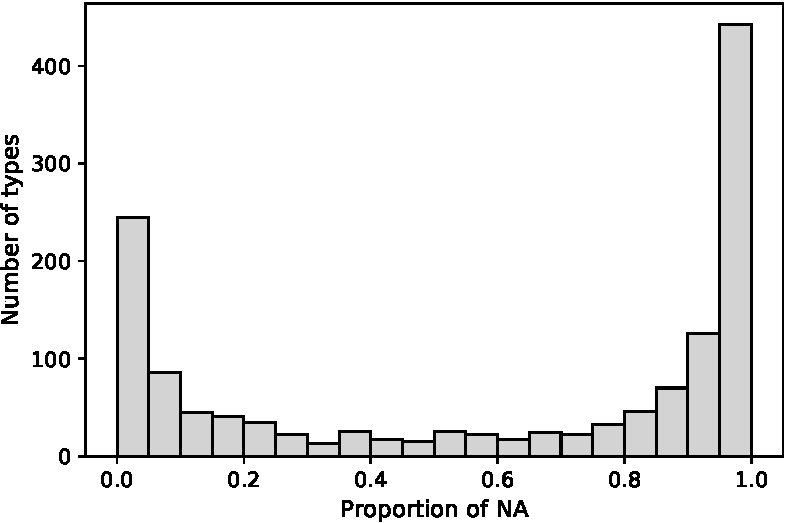
\includegraphics[scale=0.6]{figures/Strnadova-global-crop.pdf}
\caption{ Distribution of relative frequencies of triples $\langle N_1,A_d,N_2\rangle$}
\label{fig:Strnadova:graphe}
\end{figure}


\largerpage[-1]
Table \ref{tab:Strnadova:freq} presents examples for the whole spectrum of relative frequencies, ranging from a strong preference for the adjectival realization at the top (\emph{Rfreq} = 0.93 for the triple $\langle\textrm{spectacle, musical, musique}\rangle$) to a strong preference for the nominal realization at the bottom (\emph{Rfreq} = 0.06 for the triple $\langle\textrm{commission, disciplinaire, discipline}\rangle$).

\begin{table}[t]
\small
 
\begin{tabularx}{\textwidth}{XXrrl}
\lsptoprule
$N_1$&$A_d$/$deN_2$&\emph{Freq}&\emph{Rfreq}&Translation\\
\midrule
\multirow{2}{*}{\emph{spectacle}}&\emph{musical}&409&\lgc{0.93}&\multirow{2}{*}{`music show'}\\
&\emph{de musique}&31&&\\
\midrule
\multirow{2}{*}{\emph{musée}}&\emph{archéologique}	&640&\lgc{0.9}&\multirow{2}{*}{`archaeological museum'}\\
&\emph{d'archéologie}&	69&&\\
\midrule
\multirow{2}{*}{\emph{réseau}}&\emph{électrique}& 333&\lgc{0.79}&\multirow{2}{*}{`electrical grid'}\\
&\emph{d'électricité}&	87&&\\
\midrule
\multirow{2}{*}{\emph{troupe}}& \emph{théâtrale} & 347 &\lgc{0.5}& \multirow{2}{*}{`theatrical troupe'}\\
&\emph{de théâtre}& 347&&\\
\midrule
\multirow{2}{*}{\emph{situation}}&\emph{critique}&47&\lgc{0.37}&\multirow{2}{*}{`critical situation'}\\
&\emph{de crise}&78&&\\
\midrule
\multirow{2}{*}{\emph{soleil}}&\emph{automnal}&21&\lgc{0.16}&\multirow{2}{*}{`automn sun'}\\
&\emph{d'automne}&109&&\\
\midrule
\multirow{2}{*}{\emph{commission}}&\emph{disciplinaire}&15&\lgc{0.06}&\multirow{2}{*}{`disciplinary committee'}\\
&\emph{de discipline}	&226&&\\
\lspbottomrule
\end{tabularx} 
\caption{Examples of $N_1 A_d$/$N_1deN_2$ combinations with their frequencies }
\label{tab:Strnadova:freq}
\end{table}


\newpage 
Table \ref{tab:Strnadova:concurrents} shows some examples which could be considered in free variation between $A_d$ and  $deN_2$ since the relative frequency is situated between 0.4 and 0.6. For triples such as $\langle\textrm{fête, familial, famille}\rangle$ or $\langle\textrm{troupe, theâtral, theâtre}\rangle$,  adjectival and nominal realizations are equivalent.

\begin{table}

\begin{tabularx}{\textwidth}{XXrrl}
\lsptoprule
$N_1$&$A_d$/$deN_2$&\emph{Freq}&\emph{Rfreq}&Translation\\
\midrule
\multirow{2}{*}{\emph{fête}}&\emph{familiale}&102&\lgc{0.42}&\multirow{2}{*}{`family party'}\\
&\emph{de famille}&143&&\\
\midrule
\multirow{2}{*}{\emph{exposition}}&\emph{photographique}&185&\lgc{0.42}&\multirow{2}{*}{`photography exhibition'}\\
&\emph{de photographie}&258&&\\
\midrule
\multirow{2}{*}{\emph{musicien}}&\emph{talentueux}&38&\lgc{0.44}&\multirow{2}{*}{`talented musician'}\\
&\emph{de talent}&48&&\\
\midrule
\multirow{2}{*}{\emph{troupe}}& \emph{théâtrale} & 347 &\lgc{0.5}&\multirow{2}{*}{`theatrical troupe'}\\
&\emph{de théâtre}& 347&&\\
\midrule
\multirow{2}{*}{\emph{campagne}}&\emph{publicitaire}&40&\lgc{0.6}&\multirow{2}{*}{`advertising campaign'}\\
&\emph{de publicité}&27&&\\
\midrule
\multirow{2}{*}{\emph{politique}}&\emph{sécuritaire}&19&\lgc{0.44}&\multirow{2}{*}{`security policy'}\\
&\emph{de sécurité}&24&&\\
\lspbottomrule
\end{tabularx}
\caption{ Examples of strong rivals ($0,4<\textrm{Rfreq}< 0,6$)}
\label{tab:Strnadova:concurrents}
\end{table}

These strong rivals are distributed across all suffixes, as shown in Table \ref{tab:Strnadova:across-suffixe} which contains a couple of adjectives which compete with their corresponding nouns introduced by \emph{de}.

\begin{table}

\begin{tabularx}{\textwidth}{Xlr}
\lsptoprule
Suffix&{Examples of adjectives} &Count \\
\midrule
\multirow{2}{*}{\sx{aire}}&\lxm{budgétaire} `budgetary', &\multirow{2}{*}{21}\\
&\lxm{sécuritaire} `security'&\\
\midrule
\multirow{3}{*}{\sx{al}}& \lxm{architectural} `architectural',&\multirow{3}{*}{51}\\
& \lxm{automnal} `autumnal'&\\
&\lxm{musical} `musical' , \lxm{familial} `family'&\\
\midrule
\multirow{2}{*}{\sx{el}}&\lxm{concurrentiel} `competitive', &\multirow{2}{*}{20}\\
&\lxm{promotionnel} `promotional'&\\
\midrule
\sx{esque}&\lxm{carnavalesque} `carnaval'&1\\
\midrule
\multirow{2}{*}{\sx{eux}}	&\lxm{argileux} `clay', \lxm{orageux} `stormy'&\multirow{2}{*}{14}\\
& \lxm{glorieux} `glorious', \lxm{prestigieux} `prestigious'&\\
\midrule
\sx{ier}&\lxm{légumier} `vegetable', \lxm{printanier} `spring'&11\\
\midrule
\multirow{3}{*}{\sx{ique}}&\lxm{archéologique} `archaeological',  &\multirow{3}{*}{36}\\
&\lxm{informatique} `information', &\\
&\lxm{touristique} `touristic'\\
\lspbottomrule
\end{tabularx}
\caption{ Examples of strong rival adjectives sorted by suffix}
\label{tab:Strnadova:across-suffixe}
\end{table}

As has been shown, the number of cases where both realizations receive the same preference is rather low.

Remember that we focused for now on cases where the formal relationship between the denominal adjective and its base noun is straightforward. One might expect to find different results where the relationship is more opaque. This is not what we found with the lexicon containing 234 noun-adjective pairs with a formal mismatch. Table \ref{tab:Strnadova:nb-study2} presents the distribution of rivals in this category according to the type frequency and Table \ref{tab:Strnadova:idio-exos} gives some examples of combinations with their frequencies. The results on this data set present a similar U-shaped distribution as we have seen in Figure \ref{fig:Strnadova:graphe}.

\begin{table}

\begin{tabular}{lrrl}
\lsptoprule
\emph{SumFreq}&\# of types  &\multicolumn{2}{c}{Both realizations}\\
\midrule
f$\geq$0&29,884&\lgc{1713}&=\lgc{6\%}\\
f$\geq$10&3,641&\lgc{673}&=\lgc{18\%}\\
f$\geq$100&582&\lgc{140}&=\lgc{24\%}\\
f$\geq$1000&52&\lgc{19}&=\lgc{36\%}\\
\lspbottomrule
\end{tabular}
\caption{ Absolute frequencies of triples $\langle N_1,A_d,N_2\rangle$ in the corpus where $A_d$ has an idiosyncratic form}
\label{tab:Strnadova:nb-study2}
\end{table}


\begin{table}

\begin{tabular}{llrrl}
\lsptoprule
$N_1$&$A_d$/$deN_2$&\emph{Freq}&\emph{Rfreq}&Translation\\
\midrule
\multirow{2}{*}{\emph{eau}}&\emph{pluviale}&435&0.75&\multirow{2}{*}{`rain water'}\\
&\emph{de pluie}&149&&\\
\hline
\multirow{2}{*}{\emph{éclipse}}&\emph{solaire}&128&0.66&\multirow{2}{*}{`solar eclipse'}\\
&\emph{de soleil}&79&&\\
\hline
\multirow{2}{*}{\emph{stage}}&\emph{linguistique}&17&0.49&\multirow{2}{*}{`language course'}\\
&\emph{de langues}&18&&\\
\hline
\multirow{2}{*}{\emph{loisir}}&\emph{estival}&13&0.14&\multirow{2}{*}{`summer leisure'}\\
&\emph{d'été}&81&&\\
\lspbottomrule
\end{tabular}
\caption{ Examples of $N_1 A_d$ / $N_1deN_2$ with absolute and relative frequencies where $A_d$ has an idiosyncratic form}
\label{tab:Strnadova:idio-exos}
\end{table}

Overall, there are not  many cases where the adjective and the noun are used to modify the same noun: We are far from a situation of interchangeability between the two.


\section {Discussion}

% At this point, the motivation for the observed situation can be discussed.

\subsection{Grammar conditions}

The low number of strong rivals is certainly due at least in part to grammatical or semantic constraints. For example, the acceptability of the $N_1deN_2$ realization is reduced where $N_1$ is a deverbal noun. A likely explanation is that prepositional complements of deverbal nouns tend to be interpreted as realizing an argument of the noun (\ref{ex:Strnadova:visite-archéol}a), while adjectives can act as simple modifiers (\ref{ex:Strnadova:visite-archéol}b). The same $deN_2$ is fine if the head noun is not deverbal  (\ref{ex:Strnadova:visite-archéol}c).

\begin{exe}
\ex \begin{xlist} \label{ex:Strnadova:visite-archéol}
\ex ?{visite d'archéologie}\\ `visit of archaeology'
\ex {visite archéologique}\\ `archaeological visit'
\ex {laboratoire d'archéologie}\\ `archaeological laboratory'
\end{xlist}
\end{exe}

Another example of such constraints, but this time in favor of free variation, is represented by quality nouns such as \emph{exception} `exception', \emph{prestige} `prestige', \emph{talent} `talent', \emph{etc.} and derived qualifying adjectives, such as \emph{talentueux} `talented', \emph{prestigieux} `prestigious', \emph{etc.} In this case, both the PP and the adjective can be functionally equivalent as shown in (\ref{ex:Strnadova:musicien-talent}).

\begin{exe}
\ex \begin{xlist} \label{ex:Strnadova:musicien-talent}
\ex {musicien de talent}\\ `talented musician'
\ex {musicien talentueux}\\ `talented musician'
\end{xlist}
\end{exe}

With this being said, there is a large residue of examples with preference for one or the other type of modifier without any clear grammatical motivation. I consider these to be a matter of usage-based conventionalization. Therefore, in (\ref{ex:Strnadova:N1scolaire}),  the very strong preference for the given alternative — 383 \emph{versus} 1 for (\ref{ex:Strnadova:N1scolaire}a) and 62 \emph{versus} 5 for (\ref{ex:Strnadova:N1scolaire}b) — is only a matter of pure convention. In certain cases, a partial semantic specialization can be observed. This is the case for the ``false rivals" in (\ref{ex:Strnadova:sortieN2}) which do not have the same meaning.

\begin{exe}
\ex \label{ex:Strnadova:N1scolaire} \begin{xlist}
\ex {fourniture scolaire} `school supplies' / f = 383
\ex {sac d'école} `school bag'  / f = 62
\end{xlist}
\end{exe}

\begin{exe}
\ex \label{ex:Strnadova:sortieN2} \begin{xlist}
\ex {sortie scolaire} `school outing' / f = 65
\ex {sortie d'école} `end of the school day' / f = 73
\end{xlist}
\end{exe}

In conclusion, denominal adjectives and prepositional phrases with \emph{de} are not in free variation. Some cases can be explained by grammar, but conventionalization seems to be an important factor which should be studied more in detail.

\subsection{Lexical conditions}

Looking at the distributions of modifiers, the choice between adjectival or prepositional modifiers seems notably conditioned by the lexical identity of the modifying concept. Thus, if your modifier denotes `security', there is a clear preference to use a PP  \emph{de  sécurité}, while if your modifier denotes `region', then the preferred modifier will be the adjective \lxm{régional}, as shown in Figure \ref{fig:Strnadova:securitaire-regional}.

\begin{figure}
\centering\small
\begin{tabular}{cc}
\emph{de sécurité} vs. \emph{sécuritaire} 
&
\emph{de région} vs. \emph{régional}\\
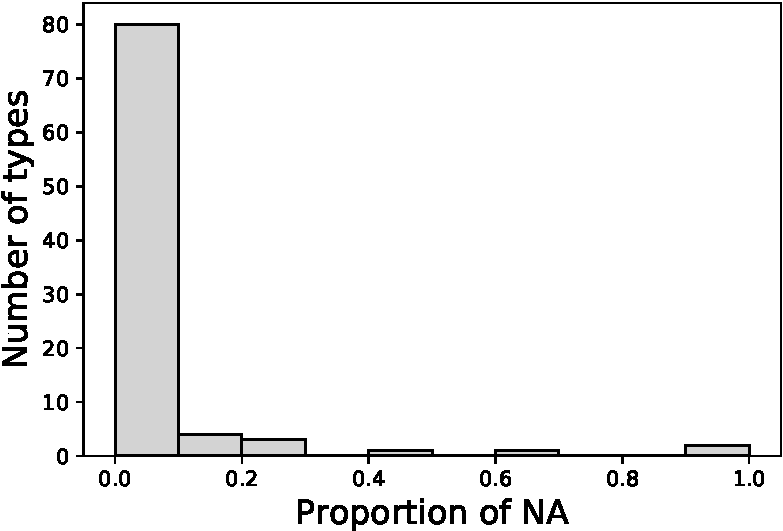
\includegraphics[scale=.4]{figures/Strnadova-securite-crop.pdf}
&
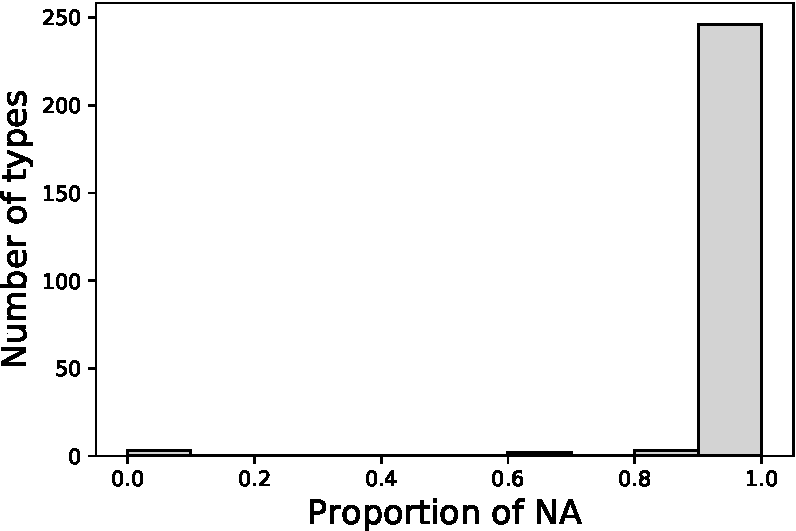
\includegraphics[scale=.4]{figures/Strnadova-region-crop.pdf}\\ \\
\end{tabular}
\caption{ Distribution of relative frequencies of triples $\langle N_1,A_d,N_2\rangle$ where $N_2$  = sécurité / région}
\label{fig:Strnadova:securitaire-regional}
\end{figure}

Each strategy has its own distribution. For example for the pairs \lxm{théâtre} `theater' / \lxm{théâtral} `theatrical' and  \lxm{musique} `music' / \lxm{musical} `musical', there is a real rivalry between the adjectival and the prepositional realization, as illustrated in Figure \ref{fig:Strnadova:theatral-musical}.

\begin{figure}
\centering\small
\begin{tabular}{cc}
\emph{de théâtre} vs. \emph{théâtral} 
&
\emph{de musique} vs. \emph{musical}\\
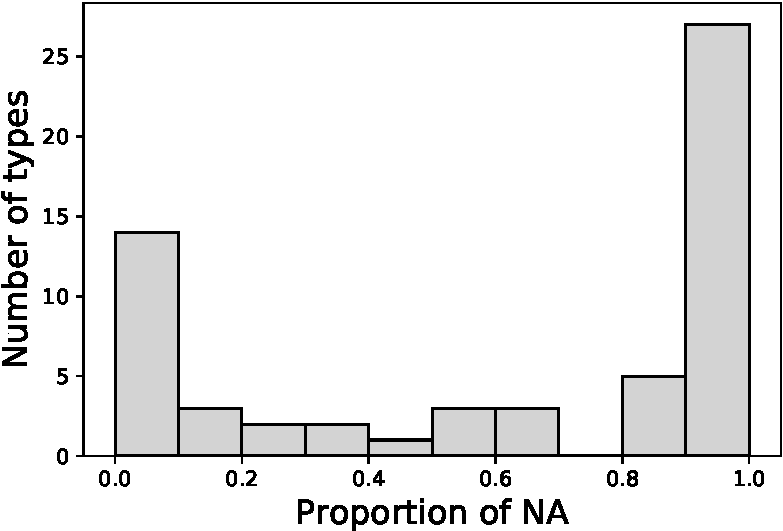
\includegraphics[scale=.4]{figures/Strnadova-theatre-crop.pdf}
&
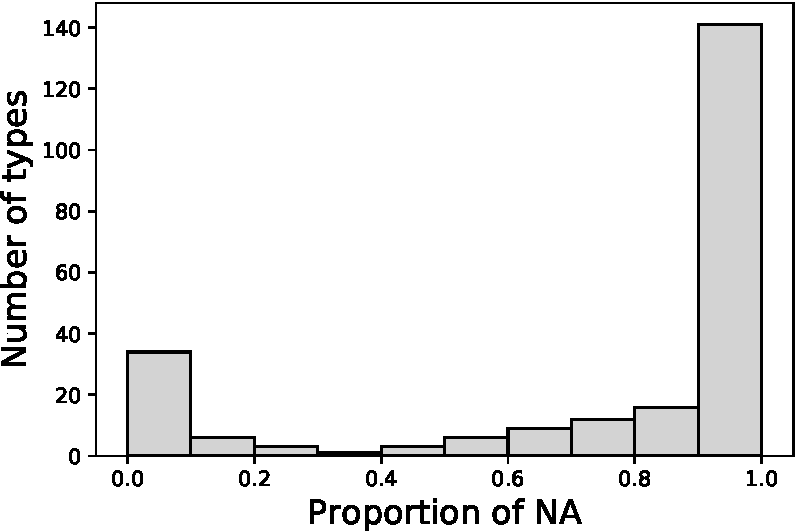
\includegraphics[scale=.4]{figures/Strnadova-musique-crop.pdf}\\ \\
\end{tabular}
\caption{ Distribution of relative frequencies of triples $\langle N_1,A_d,N_2\rangle$ where $N_2$  =  théâtre / musique}
\label{fig:Strnadova:theatral-musical}
\end{figure}

The four seasons, such as the example (\ref{ex:Strnadova:automne}), can be presented as another good example: as shown in Figure \ref{fig:Strnadova:Saisons}, the use of a PP is much more frequent than the use of denominal adjectives which are commonly used  only in a poetic register.

\begin{exe}
\ex \label{ex:Strnadova:automne} {balade d'automne / automnale} `autumn walk'
\end{exe}

\begin{figure}
\centering
\small
\begin{tabular}{cc}
\emph{de printemps} vs. \emph{printanier} 
&
\emph{d'été} vs. \emph{estival}\\
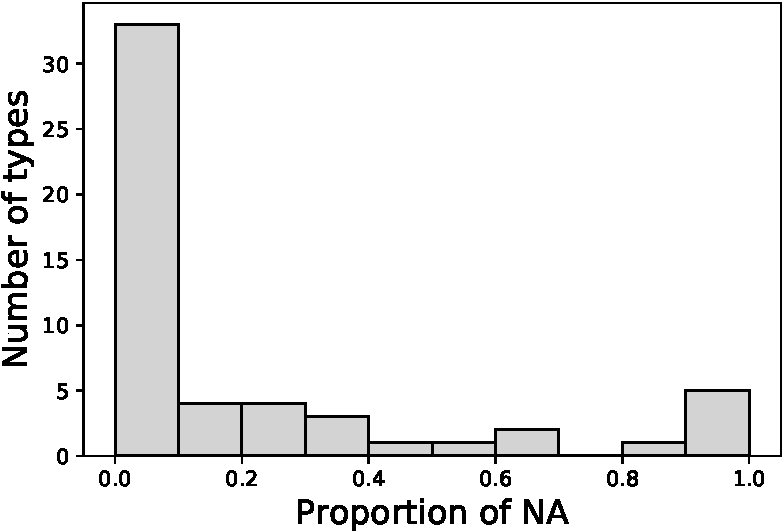
\includegraphics[scale=.4]{figures/Strnadova-printemps-crop.pdf}
&
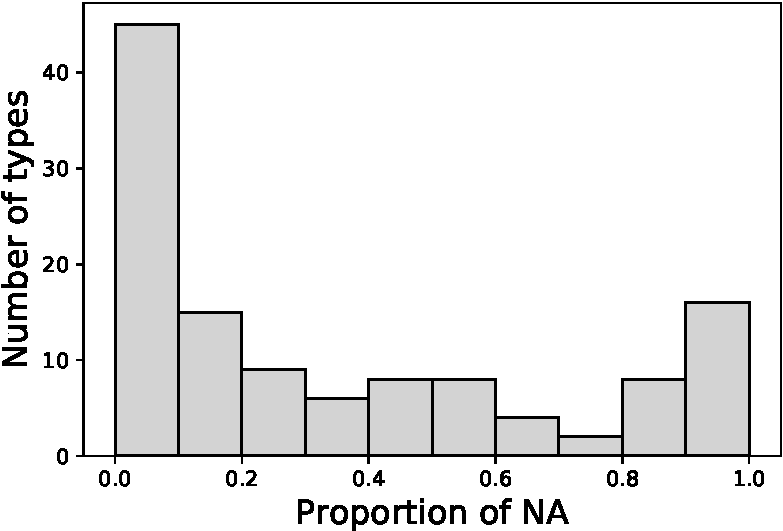
\includegraphics[scale=.4]{figures/Strnadova-estival-crop.pdf}\\ \\
\emph{d'automne} vs. \emph{automnal} 
&
\emph{d'hiver} vs. \emph{hivernal}\\
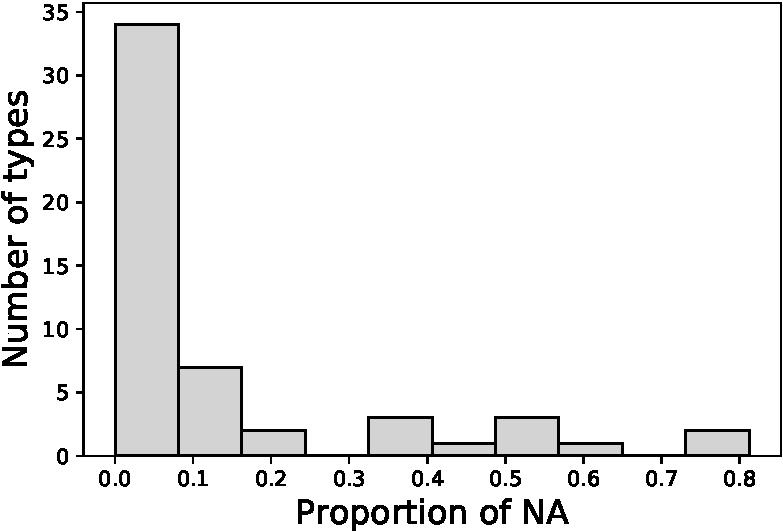
\includegraphics[scale=.4]{figures/Strnadova-automnal-crop.pdf}
&
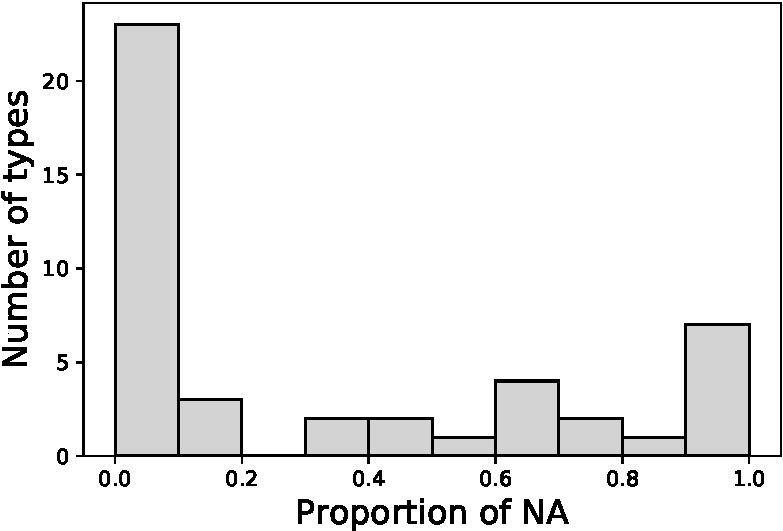
\includegraphics[scale=.4]{figures/Strnadova-hiver-crop.pdf}
\end{tabular}
\caption{ Distribution of relative frequencies of triples $\langle N_1,A_d,N_2\rangle$ where $N_2$ is a season}
\label{fig:Strnadova:Saisons}
\end{figure}

Thus, register can also play a role in the choice of the realization. This observation corresponds to the conclusion of \citet{cartonideleger2010} on medical texts where adjectives are more frequent in specialized texts than in more general texts.

Another question is to know to which extent the choice of one or the other alternative is conditioned by the identity of the head noun. For example, the nouns \emph{zone} `zone' and \emph{concours} `competition' have equally distributed adjectival and prepositional modifiers, as presented in Figure \ref{fig:Strnadova:zone-concours}. This would need to be assessed against the whole dataset taking into account the semantic relationship between the head noun and the modifying concept, for example by relying on the principles of distributional semantics.

\begin{figure}
\small
\begin{tabular}{cc}
N$_1$ is \emph{zone} 
&
N$_1$ is \emph{concours}\\
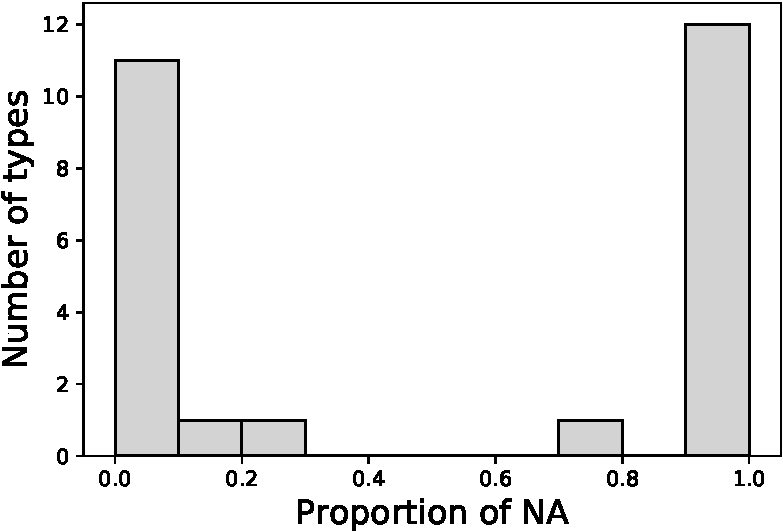
\includegraphics[scale=.4]{figures/Strnadova-zone-crop.pdf}
&
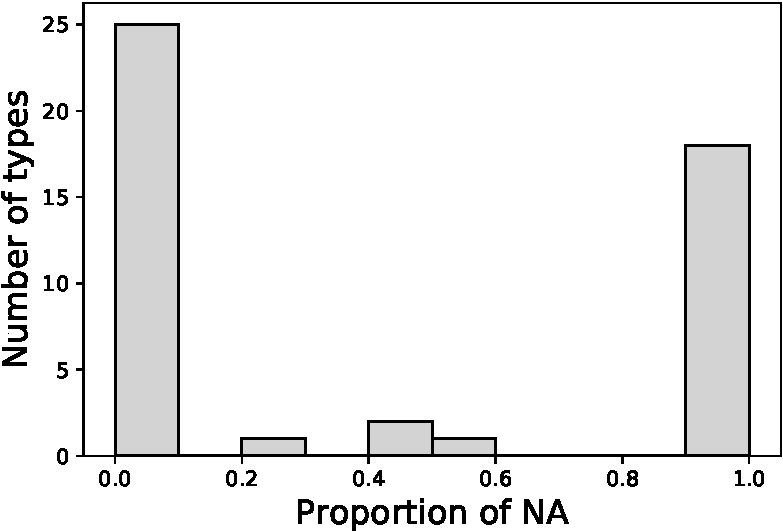
\includegraphics[scale=.4]{figures/Strnadova-concours-crop.pdf}
\end{tabular}

\caption{ Distribution of relative frequencies of triples $\langle N_1,A_d,N_2\rangle$ where $N_1$  =  zone / concours}
\label{fig:Strnadova:zone-concours}
\end{figure}

This section has shown that denominal adjectives and prepositional phrases are seldom equivalent. First, free variation is rare. Then, the lexical identity of the pair noun\rel{}adjective is decisive for the choice of the preferred realization. Finally, in many cases, this preference is purely conventional and cannot be explained in terms of grammar alone.

\section{Conclusion}

This paper questioned the purported equivalence between French denominal adjectives and morphologically related nouns embedded in prepositional phrases introduced by \emph{de}. This idea has been present in the literature since at least the 18th century. In the same way as two word forms can fill the same cell of a lexeme's inflectional paradigm or two dative constructions can alternate or a synthetic and a periphrastic form can compete for degree realization on adjectives and adverbs, there are two ways to express noun modification — with a denominal adjective or with a prepositional phrase introduced by \emph{de}. Of course, there are other linguistic means that can be used for modification, but they have not been taken for granted to the same extent.

I have shown that denominal adjectives and prepositional phrases are not in free variation (\emph{sortie scolaire / sortie d'école}). Instead, they have a U-shaped distribution with a majority of cases favoring one or the other strategy and only few cases in the middle of the distribution. In general, there is some usage-based conventionalization %(\emph{fourniture scolaire / sac d'école}) 
which is not written in any grammar rules but  learned  implicitly when learning the language. Some  language register preference may also play a role.% (\emph{balade d'automne / automnale}).

This paper presents a certain phenomenology of the question and the overview of what kinds of factors need to be taken into account and studied in more detail with respect to the choice between adjectival and nominal realization. Moreover, not only is it important to look into the rivals, but one also needs to look into the edges of the distribution: are there any specific constructions where the use of one or the other strategy can be predicted? A quick look at the data reveals that, for example, in combinations which favor nominal realization, there are cases where $N_1$ is a deverbal noun and the noun embedded in the prepositional phrase saturates its argument structure (\emph{demande de soutien} `request for support', \emph{abandon de chien} `dog abandonment') or cases where $N_2$ is a deverbal noun and there is no adjective derived from it (\emph{horaire d'ouverture} `opening hours', \emph{issue de secours} `emergency exit'). Another group that favors $N_1deN_2$ are combinations where $N_1$ is a quantity or a measure noun (\emph{vingtaine de commerçants} `twenty of shopkeepers',  \emph{tonne d'acier } `ton of steel').

\rephrase{In conclusion}{To conclude}, both denominal adjectives and nouns embedded in prepositional phrases with \emph{de} can be used as modifiers, but they usually do not have the same distribution or the same meaning. This brings us to a more theoretical question: could a prepositional phrase be considered as a possible candidate for the \emph{modifier} cell of a derivational paradigm? As could be seen, especially nouns for which there is no corresponding derived adjective would have this cell empty for a synthetic form, but they could have it filled with a prepositional phrase. This could be considered as a sort of periphrasis, in a very similar way as inflectional paradigms contain synthetic and periphrastic forms. The results of our corpus study suggest that extending this possibility to all lexemes would bring many new challenges.


{\sloppy
    \printbibliography[heading=subbibliography,notkeyword=this]
}


\end{document}
